
% Solutions to exercises in Paolo Aluffi's "Algebra: Chapter 0"
% All solutions copyright 2015 Shane Creighton-Young

% The scrartcl document class lets us have a wider stroke width for the fonts. However, it
% changes the heading font by default so we've used the \setkomafont command to
% restore the headings to the vanilla LaTeX style.
\documentclass[fontsize=14pt]{scrartcl}
\setkomafont{disposition}{\normalfont\bfseries}

% Standard American Math Society packages provide theorem environments, symbols,
% etc.
\usepackage{amsthm}
\usepackage{amsmath}
\usepackage{amssymb}

% For including graphics (such as charts and diagrams.)
\usepackage{graphicx}
\graphicspath{ {.} }

% Add lcm operator.
\DeclareMathOperator{\lcm}{lcm}

% The tiks-cd package provides macros for easily writing commutative diagrams.
% For more info see [1].
% [1]: http://ctan.math.ca/tex-archive/graphics/pgf/contrib/tikz-cd/tikz-cd-doc.pdf
\usepackage{tikz-cd}

% The pdfrender package is used to output fonts with a larger stroke width.
\usepackage{pdfrender}

% The mathrsfs package provides the script font.
\usepackage{mathrsfs}

\usepackage[margin=0.6in]{geometry}

% The chngcntr ("change counter") package is used here so that subsection
% numbers are written without the leading section number. This takes place in
% the subsection headings as well as the theorem environment numbering.
%
% Before:
% 1. Section
% 1.1. Subsection
% Problem 1.1.1. What is 1 + 1?
% Problem 1.1.2. What is 1 + 2?
%
% After:
% 1. Section
% 1. Subsection
% Problem 1.1. What is 1 + 1?
% Problem 1.2. What is 1 + 2?
\usepackage{chngcntr}
\counterwithout{subsection}{section}

% The problem environment is a regular ams theorem environment with "Problem"
% text and some leading space to give some separation between the problems.
\theoremstyle{definition}
\newtheorem{problem-internal}{Problem}[subsection]
\newenvironment{problem}{
  \medskip
  \begin{problem-internal}
}{
  \end{problem-internal}
}

% The solution environment is a proof environment with the "solution" text as
% well as the following adjustments:
% - No indent on paragraphs;
% - A small amount of space between paragraphs.
%
% Note: The negative space at the beginning is to remove the space before the
% first paragraph in the solution.
\newenvironment{solution}{
  \begin{proof}[Solution]
  \vspace{-8px}
  \setlength{\parskip}{4px}
  \setlength{\parindent}{0px}
}{
  \end{proof}
}

% Renewing the \thesection command changes the section numbers to roman
% numerals. This matches the style of the Aluffi textbook.
%
% Before:
% 1. Section
% 1.1. Subsection
%
% After:
% I. Section
% I.1. Subsection
\renewcommand{\thesection}{\Roman{section}} 

% Allow linebreaks at commas
% http://tex.stackexchange.com/questions/1959/allowing-line-break-at-in-inline-math-mode
\makeatletter
\def\old@comma{,}
\catcode`\,=13
\def,{%
  \ifmmode%
    \old@comma\discretionary{}{}{}%
  \else%
    \old@comma%
  \fi%
}
\makeatother

% Set with spacing padding for the curly braces.
\newcommand{\set}[1]{\left\{\,#1\,\right\}}
\newcommand{\id}{\mathrm{id}}
\newcommand{\im}{\mathrm{im}}
\newcommand{\Obj}{\mathrm{Obj}}
\newcommand{\Hom}{\mathrm{Hom}}
\newcommand{\Grp}{\mathsf{Grp}}
\newcommand{\Set}{\mathsf{Set}}
\newcommand{\Ab}{\mathsf{Ab}}
\newcommand{\abs}[1]{\left|#1\right|}
% Inuitive "from" command draws an arrow pointing left, A <- B reads "A from p"
\newcommand{\from}{\leftarrow}
\newcommand{\quotuniv}[1]{\overline{#1}}
% inverses should have a -1
\newcommand{\inv}[1]{#1^{-1}}
% typesets the cyclic group of size #1
\newcommand{\cycl}[1]{\mathbb{Z}/#1\mathbb{Z}}

\begin{document}



\section*{Chapter 2: Groups, first encounter}
\subsection{Definition of group}


% Problem 1.1
\begin{problem}
Write a careful proof that every group is the group of isomorphisms of a
groupoid. In particular, every group is the group of automorphisms of some
object in some category. (\S2.1]
\end{problem}
\begin{solution}
\def \C {\mathsf{C}}
Let $G$ be a group with binary operation $\circ$ and identity $e$. Consider a
category $\C$ with a single object $\emptyset$. We will show that the elements
of $G$ make suitable morphisms $\Hom_\C(\emptyset,\emptyset)$ with $\circ$ as a
composition operation.

Since $G$ is a group, $G$ (i.e. $\Hom_\C(\emptyset,
\emptyset)$) is closed $\circ$ and $\circ$ is transitive for morphisms. The
identity $e$ makes an appropriate identity morphism for $\emptyset$. Hence $\C$
is a category.

Lastly, we will show that $\C$ is a groupoid. Any morphism
$f\in\Hom_\C(\emptyset, \emptyset)$ has a (two-sided) inverse $\inv{f}$ since $G$
is a group. This means that $f$ is an isomorphism.
\end{solution}


% Problem 1.2
\begin{problem}
Consider the `sets of numbers' listed in \S1.1, and decide which are made into
groups by conventional operations such as $+$ and $\cdot$. Even if the answer is
negative (for example, $(\mathbb{R},\cdot)$ is not a group), see if variations
on the definition of these sets lead to groups (for example,
$(\mathbb{R}^*,\cdot)$ is a group; cf. \S1.4). [\S1.2]
\end{problem}
\begin{solution}
This is open-ended, so I don't want to do it.
\end{solution}

\begin{problem}
Prove that $\inv{(gh)} = \inv{h}\inv{g}$ for all elements $g,h$ of a group $G$.
\end{problem}
\begin{solution}
Let $B$ be a group and suppose $f,g\in G$. Then we have:
%
\[ (\inv{g}\inv{f})(fg) = (\inv{g}(\inv{f}f))g = (\inv{g}e)g = \inv{g}g = e \]
\[ (fg)(\inv{g}\inv{f}) = (f(g\inv{g}))\inv{f} = (fe)\inv{f} = f\inv{f} = e \]
%
Hence $\inv{g}\inv{f}$ is a two-sided inverse of $gf$.
\end{solution}


% Problem 1.3
\begin{problem}
Suppose that $g^2 = e$ for all elements $g$ of a group $G$; prove that $G$ is
commutative.
\end{problem}
\begin{solution}
Let $G$ be a group such that for all $g\in G$ we have $g^2=e$. Fix $g,h\in G$.
Then,
%
\[ gh = eghe = hhghgg = h(hg)^2g = hg \]
%
as required.
\end{solution}


% Problem 1.4
\begin{problem}
The `multiplication table' of a group is an array compiling the results of all
multiplications $g\bullet h$:

[Redacted.]

(Here $e$ is the identity element. Of course the table depends on the order in
which the elements are listed in the top row and leftmost column.) Prove that
every row and every column of the multiplication table of a group contains all
elements of the group exactly once (like Sudoku diagrams!).
\end{problem}
\begin{solution}
Without loss of generality suppose that two elements in a column are different,
i.e. for some fixed element $f$ we have $f\bullet g = f\bullet h$. Then by
(left-)cancellation we get that $g=h$. Hence the columns must be the same.
\end{solution}


% Problem 1.5
\begin{problem}
$\neg$ Prove that there is only one possible multiplication table for $G$ if $G$
has exactly 1, 2, or 3 elements. Analyze the possible multiplication tables for
groups with exactly 4 elements, and show that there are two distinct tables, up
to reordering the elements of $G$. Use these tables to prove that all groups
with $< 4$ elements are commutative.

(You are welcome to analyze groups with 5 elements using the same technique, but
you will soon know enough about groups to be able to avoid such brute-force
approaches.) [2.19]
\end{problem}
\begin{solution}
(Note: I spent a lot of time trying to figure out why there seemed to be many
more than 2 tables for groups with exactly 4 elements until going back to the
question where it there are only 2 ``up to reordering''!)

If a group only has one element, say $G=\set{e}$, there is only one spot to fill.
Since multiplication must be closed it must be $e$. Here $e$ is the identity.

If a group has two elements, say $G=\set{e,g}$, then there are four spots to
fill. The $e$-row and $e$-column are easy, so there is only one non-trivial
column to fill. If $gg=g$ then by cancellation we get that $g=e$, which is a
contradiction since $g$ is distinct from $e$. So $gg=e$.

Suppose that $G=\set{e,g,h}$. Here there are four non-trivial spots to fill.  We
can't have that $gh=h$ (by cancellation as above), so we must have $gh=e$. For
the same reason, we must have $hg=e$. There is no other choice but to set
$g^2=h$ and $h^2=g$.

Suppose that $G=\set{e,f,g,h}$. This is the tricky one. There are nine spots to
fill. First of all, we note that due to the double-sidedness of inverses, we
have that for $f,g,h\in G$ (all distinct) we can't have that $fg=h$ and $gf=e$
(the second implies that $f=\inv{g}$, but then the first says $\inv{g}{g}\neq
e$, a contradiction.) This in fact implies commutativity, since for any distinct
$f,g\in G$ it must either be the case that $fg=e=gf$ or $fg=h=gf$.

The question states that there are only two ``up to the order of the elements''.
So, rather than answer ``how many possible tables are there'', we will answer:
how many $n$ are such that $n$ elements of $G$ go to the identity when squared?
We'll see that only $n=1$ and $n=3$ work; and that the only differences in the
tables for $n=1$ are the choosing of which element has order 2 (i.e. which
element goes to the identity when it is squared;) and that there is only one
table where $n=3$.

Clearly it can't work for $n<0$ or $n>3$ (we can't choose less than 0 or more
than 3 elements from $G$.) We claim that it can't be that no element in $G$ has
order 2. To see this, without loss of generality consider $f$. We know that $f$
must have an inverse that is distinct from itself (or else we get an immediate
contradiction) and from $e$---without loss of generality, suppose $\inv{f}=h$.
This also means that $\inv{h}=f$.  Now we ask: which element can be the inverse
of $g$? It can't be $f$ or $h$ because the inverse is unique and $g$ is distinct
from $f$ and $h$. It also can't be $e$ since $ge=g$ by definition.  So it must
be $g$. But this means that there are 1 elements that have order 2.  We have
shown that, if any element in $G$ doesn't have order 2, another must have order
2. So zero order two elements is a contradiction.

Now we claim that having only two elements of order not equal to 2 is also
infeasible. Assume without loss of generality that $f^2=e$ and $g^2=e$. What is
$h^2$? We note that the inverse of $h$ cannot be $e$ by cancellation, and cannot
be $f$ or $g$ since inverses are unique and $h$ is distinct from $f$ and $g$.
This means that $h$ must be its own inverse, and thus has order 2. Therefore,
two elements of order 2 implies three elements of order 2.

Now we'll show that one order 2 element works okay. Without loss of generality
assume $f^2=e$. Here we must take $gh=hg=e$. These are three cells in our table.
Furthermore, we must have $fg=h$ (since $fg$ can't be $f$ or $g$ or $e$), and
similarly for $fh=g$. By commutativity we also have that $gf=h$ and $hf=g$. Now
we've filled seven cells in our table. By our above ``theorem'' about column and
row uniqueness we know we must take $gh=hg=f$. Hence there is only one group of
size 4 with only one order 2 element (up to the selection of which element has
order 2.)

Last, consider the group of size 4 where all elements are order 2. Immediately
we deducate that $fg=h$ (since it can't be $e$, $f$, or $g$ by cancellation,)
and then that $fh=g$ (since it is the last option!) Similarly that $gh=f$, and
so on---there is only one group where all elements are order 2.
\end{solution}


% Problem 1.7
\begin{problem}
Prove Corollary 1.11.
\end{problem}
\begin{solution}
Too easy: $\abs{g}$ is a divisor of $n$ is equivalent to $n$ is a multiple of
$\abs{g}$.
\end{solution}


% Problem 1.8
\begin{problem}
Let $G$ be a finite group, with exactly one element $f$ of order 2. Prove that
$\prod_{g\in G}g = f$. [4.16]
\end{problem}
\begin{solution}
I struggled a lot with this problem. The question implies that $\prod_{g\in G}$
is well-defined, which means that $G$ is a commutative group, however I could
not prove this.

Assuming that it is commutative, then we can take $G=\set{e, f, g_1, \dots, g_m,
\inv{g_1}, \dots, \inv{g_m}}$ all distinct. Then the product $\prod_{g\in G}$,
since $G$ is commutative, can be written $efg_1\inv{g_1}\cdots
g_m\inv{g_m}=efe\cdots e = f$ as required.

(I hope to figure out how to prove that $G$ is commutative eventually.)
\end{solution}


% Problem 1.9
\begin{problem}
Let $G$ be a finite group, of order $n$, and let $m$ be the number of elements
$g\in G$ of order exactly 2. Prove that $n - m$ is odd. Deduce that if $n$ is
even, then $G$ necessarily contains elements of order 2.
\end{problem}
\begin{solution}
Let $G$, $n$, $m$ as above. Note that every element $g\in G$ that is not $e$ and
is not order 2 has a unique inverse $\inv{g}$ such that $g\neq \inv{g}$. Hence
every element except for $e$ and except for all the order 2 elements come in
pairs; there are, say $2k$ of them. Then $n=1+m+2k$, where the 1 corresponds to
$e$, $m$ is the number of order-2 elements, and $k$ is the number of pairs
$g,\inv{g}$. It follows that $n-m=2k+1$, so $n-m$ is odd.

Further, suppose $n$ is even, so $n=2p$ for some $p$ with $p>k$ (for the $2k$
elements doesn't include the identity element $e$, there must be more than $2k$
elements in $G$, i.e. $2p>2k$, which implies $p>k$.) Then $n=2p=1+m+2k$.
Rearranging we get that $m=2(p-k)-1$. Since $p>k$, $p-k\geq 1$, so $2(p-k)\geq
2$, and $2(p-k)-1\geq 1$, hence $m\geq 1$ so $G$ necessarily contains at least
one element of order 2.
\end{solution}


% Problem 1.10
\begin{problem}
Suppose the order of $g$ is odd. What can you say about the order of $g^2$?
\end{problem}
\begin{solution}
Suppose $\abs{g}=2k+1$ for some $k$. Then, by Proposition 1.13,
%
\[ \abs{g^2} = \frac{\lcm(2,2k+1)}{2} = \frac{4k+2}{2} = 2k+1 \]
%
(where we take $\lcm(2,2k+1)=2(2k+1)$ since $2k+1$, being odd, is relatively
prime with $2$.) Hence $\abs{g^2}=\abs{g}$.
\end{solution}


% Problem 1.11
\begin{problem}
Prove that for all $g$, $h$ in a group $G$, $\abs{gh} = \abs{hg}$. (Hint: Prove
that $\abs{\inv{a}ga} = \abs{g}$ for all $a$, $g$ in $G$.)
\end{problem}
\begin{solution}
Let $g,a\in G$. Suppose $\abs{g}=n$. Then,
%
\[ (\inv{a}ga)^n = (\inv{a}ga)(\inv{a}ga)\cdots(\inv{a}ga) =
\inv{a}g(a\inv{a})g\cdots g(a\inv{a})ga = \inv{a}g^na \]
%
We also have that $g^n = e \iff g^n = a\inv{a} \iff \inv{a}g^na=e$. This means
that $\abs{\inv{a}ga}= n = \abs{g}$, which implies that $\abs{ag} =
\abs{a\inv{a}ga} = \abs{ga}$, as required.
\end{solution}


% Problem 1.12
\begin{problem}
I don't want to typeset the matrices!
\end{problem}


% Problem 1.13
\begin{problem}
$\rhd$ Give an example showing that $\abs{gh}$ is not necessarily equal to
$\lcm(\abs{g}, \abs{h})$, even if $g$ and $h$ commute. [§1.6, 1.14]
\end{problem}
\begin{solution}
Consider the 4-group with 1 element of order two as above. Then we have
$G=\set{e,f,g,h}$ with $f^2=e$, $gh=hg=e$, and $g^2=h^2=f$. Here we have that
$\abs{gh}=\abs{e}=0$, while $\lcm(\abs{g},\abs{h})=\lcm(4,4)=4$, so
$\abs{gh}\neq\lcm(\abs{g},\abs{h})$. 
\end{solution}


% Problem 1.14
\begin{problem}
$\rhd$ As a counterpoint to Exercise 1.13, prove that if $g$ and $h$ commute and
$\gcd(\abs{g}, \abs{h}) = 1$, then $\abs{gh}=\abs{g}\abs{h}$. (Hint: Let $N =
\abs{gh}$; then $g^N = (\inv{h})^N$. What can you say about this element?) [\S
1.6, 1.15, \S IV.2.5]
\end{problem}
\begin{solution}
Let $g,h\in G$ with $gh=hg$. Set $\abs{g}=n$, $\abs{h}=m$, and
$\abs{gh}=\abs{hg}=N$. Suppose that $\gcd(n,m)=1$. We have by Proposition 1.14
that $N\mid\lcm(n,m)$. Since $\gcd(n,m)=1$, $\lcm(n,m)=nm$. So $nm=kN$ (1) for
some $k$. Also, since $\gcd(n,m)=1$ we get that $N\mid n$ xor $N\mid m$.
Suppose, without loss of generality, that $N\mid n$, so that $n=\ell N$ for some
$\ell$ (2). Divide (1) by (2) to get that $m=\frac{k}{\ell}$ (3).

Now, we will prove that $k=1$. Since $(gh)^N=g^N=e$, we get that
$g^N=(\inv{h})^N$ (4). By (2) we get that $\abs{g^N}=\ell$. Since $h^m=e$, we have
$hh^{m-1}=e$, so $\inv{h}=h^{m-1}$. By (4) we know that
$\abs{(h^{m-1})^N}=\abs{h^{N(m-1)}}=\ell$. However, by Proposition 1.13 we know
that $\ell =\frac{\lcm(m,N(m-1))}{N(m-1)}$. Since $N\mid nm$ and $\gcd(n,m)=1$
and we're assuming $N\mid n$, $\gcd(N,m)=1$. So
$\ell=\frac{m(N(m-1))}{N(m-1)}=m$. From this we get $m = \frac{k}{\ell} =
\frac{k}{m} \implies k=1$. Looking back at (1) where $nm=kN$ we can finally
deduce that $nm=N$.
\end{solution}


% Problem 1.15
\begin{problem}
$\neg$ Let $G$ be a commutative group, and let $g\in G$ be an element of maximal
finite order, that is, such that if $h\in G$ has finite order, then
$\abs{h}<\abs{g}$.  Prove that in fact if $h$ has finite order in $G$, then
$\abs{h}\mid\abs{g}$. (Hint: Argue by contradiction.  If $\abs{h}$ is finite but
does not divide $\abs{g}$, then there its a prime integer $p$ such that $\abs{g}
= p^mr$, $\abs{h} = p^ns$, with $r$ and $s$ coprime to $p$ and $m < n$. Use
Exercise 1.14 to compute the order of $g^{p^m}h^s$.) [\S 2.1, 4.11, IV.6.15]
\end{problem}
\begin{solution}
Let $G$ be a commutative group and suppose $g\in G$ has maximal finite order.
Let $h\in G$.  Let $\abs{g}=m$, $\abs{h}=n$. Suppose for contradiction that
$n\nmid m$. So $n>1$ and there is a prime $p$ such that $m=p^kr$ and $n=p^\ell
s$ with $0\leq k < \ell$ and $\gcd(p,r)=\gcd(p,s)=1$. Consider $g^{p^k}h^s$.
Using Proposition 1.13, we calculate the order of each element:
%
\[ \abs{g^{p^k}} = \frac{\lcm(p^k,m)}{p^k} = \frac{m}{p^k} = r \]
\[ \abs{h^s} = \frac{\lcm(s,n)}{s} = \frac{n}{s} = p^\ell \]
%
Now, by Exercise 1.14 above, and since $G$ is a commutative group and since
$\gcd(r,p^\ell) = 1$, we get that $\abs{g^{p^k}h^s} = \abs{g^{p^k}}\abs{h^s} =
rp^\ell$. However, since $k<\ell$, $\abs{g}=m=p^kr<p^\ell r$, contradicting the
maximality of $\abs{g}$. This means that for all primes $p$, its multiplicity in
the factorization of $\abs{g}$ must be greater than that of $\abs{h}$; i.e.
$k\geq\ell$ for all primes $p$. This means that $\abs{h}$ divides $\abs{g}$ as
required.
\end{solution}



\subsection{Examples of groups}


% Problem 2.1
\begin{problem}
$\neg$ One can associate an $n\times n$ matrix $M_\sigma$ with a permutation
$\sigma\in S_n$, by letting the entry at $(i, \sigma(i))$ be 1 and letting all
other entries be 0.  [Redacted example.] Prove that, with this notation,
%
\[ M_{\sigma\tau} = M_\sigma M\tau \]
%
for all $\sigma,\tau\in S_n$, where the product on the right is the ordinary
product of matrices.
[IV.4.13]
\end{problem}
\begin{solution}
Let $n\in\mathbb{N}$. Suppose $\sigma,\tau\in S_n$. We need to verify that, for
each $k\in\set{1,\dots,n}$, $(M_\sigma M_\tau)_{k,\sigma\tau(k)}=1$, and
$(M_\sigma M_\tau)_{i,\sigma\tau(k)}=0$ for all $i\neq k$. So, let
$k\in\set{1,\dots, n}$. First we calculate the value at $(k,\sigma\tau(k))$ in
$M_\sigma M_\tau$:
%
\begin{align*}
&\,\,  \sum_{i=0}^n (M_\sigma)_{k,i} (M_\tau)_{i,\sigma\tau(k)} \\
=&\,\, (M_\sigma)_{k,\sigma(k)} (M_\tau)_{\sigma(k),\sigma\tau(k)}
\end{align*}
%
Since every entry in the $k$-th row of $M_\sigma$ is 0 except for the
$\sigma(k)$-th row, which is 1, by definition. Now, if $\ell=\sigma(k)$, then
$(M_\tau)_{\sigma(k),\sigma\tau(k)} = (M_\tau)_{\ell, \tau(\ell)} = 1$, by
definition, so the entry in $M_\sigma M_\tau$ is 0 as required.

Further, the value $(m,\sigma\tau(k)$ where $m\neq k$ is 
%
\begin{align*}
&\,\,  \sum_{i=0}^n (M_\sigma)_{m,i} (M_\tau)_{i,\sigma\tau(k)} \\
=&\,\, (M_\sigma)_{m,\sigma(m)} (M_\tau)_{\sigma(m),\sigma\tau(k)}
\end{align*}
%
and since $m\neq k$, $(M_\tau)_{\sigma(m),\sigma\tau(k)}=0$. This shows is that
composing the two permutations $\sigma$ and $\tau$ is the same as multiplying
the associated matrices $M_\sigma$ and $M_\tau$.
\end{solution}


% Problem 2.2
\begin{problem}
$\rhd$ Prove that if $d < n$, then $S_n$ contains elements of order $d$. [\S2.1]
\end{problem}
\begin{solution}
Let $n,d\in\mathbf{N}$ with $d\leq n$. Consider $\sigma_d\in S_n$, defined as
\begin{align*}
\sigma_d(k) &= k+1& \text{ if $k\in\set{1,\dots,d-1}$} \\
\sigma_d(k) &= 1&   \text{ if $k=d$} \\
\sigma_d(k) &= k&   \text{ otherwise.}
\end{align*}
Now, let $k\in\set{1,\dots,n}$. We claim that $\sigma_d^d(k)=k$. If $d<k$, then
$\sigma_d^d(k)=\sigma_d(k)=k$, i.e. $\sigma_d$ has no effect on $k$. Otherwise,
let $\ell=d-k>1$. We get the following cycle:
\begin{align*}
\sigma_d(k) &= k+1 \\
\sigma_d^2(k) &= k+2 \\
&\vdots \\
\sigma_d^\ell(k) &= d \\
\sigma_d^{1+\ell}(k) &= 1 \\
\sigma_d^{2+\ell}(k) &= 2 \\
&\vdots \\
\sigma_d^{(k-1)+\ell}(k) &= k-1 \\
\sigma_d^{k+\ell}(k) &= \sigma_d^{d}(k) = k
\end{align*}
hence $\sigma_d^d=\iota_n=e_{S_n}$ as required.
\end{solution}


% Problem 2.3
\begin{problem}
For every positive integer $n$ find an element of order $n$ in $S_\mathbb{N}$.
\end{problem}
\begin{solution}
We use the above construction $\sigma_d$; it also works as a permutation in
$S_\mathbb{N}$, except it has a larger set for its domain and codomain. We also
proved that it has order $n$, so we're done.
\end{solution}


% Problem 2.4
\begin{problem}
Define a homomorphism $D_8\to S_4$ by labeling vertices of a square, as we did
for a triangle in \S2.2. List the 8 permutations in the image of this
homomorphism.
\end{problem}
\begin{solution}
I did it! I'm not going to typeset them here, but in performing this exercise I
found an error in the text. It defines the reflections in $D_{2n}$ to be all the
reflections ``about a line through each vertex and the origin.'' However, this
only covers half of them for polygons with an even number of vertices! For even
polygons we get $n/2$ reflections using lines created with vertices (since each
such line covers not one but \textit{two} vertices), and we have to use the
midpoints of edges to get the other $n/2$ reflections (they come in pairs as
well.)
\end{solution}


% Problem 2.5
\begin{problem}
$\rhd$ Describe generators and relations for all dihedral groups $D_{2n}$.
(Hint: Let $x$ be the reflection about a line through the center of a regular
$n$-gon and a vertex [in this case, since we only need \textit{one} reflection,
it is correct to say ``a vertex'' and not ``a vertex or an edge;'' however, it
could also be a reflection over an edge,] and let $y$ be the counterclockwise
rotation by $2\pi/n$. The group Den will be generated by $x$ and $y$, subject to
three relations14. To see that these relations really determine $D_{2n}$, use
them to show that any product $x^{i_1}y^{j_1}\cdots x^{i_n}y^{j_n}$ equals
$x^ry^s$ for some $r$,$s$ with $0\leq r<1$ and $0\leq s<n$.) [8.4, \S IV.2.5]
\end{problem}
\begin{solution}
Let $n\in\mathbb{N}$ and consider $D_{2n}$. Let $x$ be the reflection about the
line between a vertex and the origin. Let $y$ be a counterclockwise rotation by
$2\pi/n$ The relations are $x^2=e$, $y^n=e$, and $yx=x^{n-1}$. Consider
$z=x^{i_1}y^{j_1}\cdots x^{i_n}y^{j_n}$ with
$i_1,j_1,\dots,i_n,j_n\in\mathbb{N}$.

We claim that the following statement $P(k)$ is true for $k=n-1,\dots,1,0$: $z$
can be written in the form $x^{i_1}y^{j_1}\cdots x^{i_k}y^{j_k}x^ry^s$ where
$0\leq r\leq 1$ and $0\leq s<n$. We will prove that it is true for $k=n$, and
then show that, for all $1\leq k\leq n$, $P(k)\implies P(k-1)$. This will allow
us to deduce that $P(0)$ is true, which is the desired result.

First, fix $k=n$. Then since $i_n,j_n$ are positive integers, we can write them
as
%
\[ i_n = 2k + r \]
\[ j_n = n\ell + s\]
%
with $0\leq r\leq 1$ and $0\leq s<n$. Then we have,
\begin{align*}
x^{i_n}y^{j_n} &= x^{2k}x^ry^{n\ell}y^s \\
&= (x^2)^kx^r(y^n)^\ell y^s \\
&= x^ry^s
\end{align*}
%
So $z$ can be written $x^{i_1}y^{j_1}\cdots x^{i_{n-1}}y^{j_{n-1}}x^ry^s$ with
appropriate $r,s$. Hence $P(n-1)$ is true.

Now, fix $k$ such that $1\leq k\leq n-1$ and assume $P(k)$. This means that
%
\begin{align*}
z &= x^{i_1}y^{j_1}\cdots x^{i_n}y^{j_n} \\
  &= x^{i_1}y^{j_1}\cdots x^{i_k}y^{j_k}x^ry^s 
\end{align*}
with $0\leq r\leq 1$ and $0\leq s<n$. Let $a=\min(j_k,r)$. Note that $0\leq
j_k,r\implies 0\leq a$, and that $r\leq 1\implies a\leq 1$. So either $a=0$ or
$a=1$.

If $a=0$, then either $j_k=0$ or $r=0$. If $j_k=0$, then we have 
\begin{align*}
x^{i_k}y^{j_k}x^ry^s &= x^{i_k+r}y^s
&= x^{r'}y^s
\end{align*}
(where $r'$ is obtained using the same division process as above.) On the other
hand, if $r=0$, then we get:
\begin{align*}
x^{i_k}y^{j_k}x^ry^s &= x^i_ky^{j_k+s}
&= x^ry^{s'}
\end{align*}
(where $s'$ is obtained using the division process.) Now, in the last case, we
have that $a=1$. This means that $r=1$ and $j_k=1$. We apply rule 3 $j_k$ times:
\begin{align*}
x^{i_k}y^{j_k}x^ry^s &= x^{i_k}y^{j_k-1}(yx)y^s \\
&= x^{i_k}y^{j_k-1}xy^{s+n-1} \text{ (once)} \\
&= x^{i_k}y^{j_k-2}xy^{s+2(n-1)} \text{ (twice)} \\
&\vdots \\
&= x^{i_k}(yx)y^{s+(j_k-1)(n-1)} \\
&= x^{i_k+1}y^{s+j_k(n-1)} \text{ ($j_k$-th time)}\\
&= x^{r'}y^{s'}
\end{align*}
where the very last step applies the division algorithm to get $0\leq r'\leq 1$
and $0\leq s'<n$. Therefore, $P(k-1)$ is true.

The result is proved since $P(n-1)\implies P(n-2)\implies\cdots \implies
P(1)\implies P(0)$, as required.
\end{solution}


% Problem 2.6
\begin{problem}
For every positive integer n construct a group containing two elements g, h.
such that [g] = 2, IhI = 2, and ugh[ = n. (Hint: For n > 1, D2n will do.)
[§1.6]
\end{problem}
\begin{solution}
For $n=1$, use $D_6$ and take $g=h=x$ (where $x$ is the generator element that
is a reflection about a point.) This way, $\abs{g}=\abs{h}=2$ and
$\abs{gh}=\abs{e}=1$ as required.

For $n>1$, use $D_{2n}$. Consider the generator elements $x$ and $y$ and the
relations $x^2=e$, $y^n=e$, and $yx=xy^{n-1}$; we take $g$ and $h$ in terms of
these. In particular, $g=y^{n-1}x$ and $h=x$. Trivially, since $h^2=x^2=e$, so
$\abs{h}=2$. For $g$, we have:
\begin{align*}
g^2 &= y^{n-1}xy^{n-1}x \\
&= y^{n-2}(yx)y^{n-1}x \\
&= y^{n-2}xy^{2(n-1)}x \text{ (by relation 3)} \\
&\vdots
&= xy^{n(n-1)}x = x(y^n)^{n-1}x = x^2 = e
\end{align*}
Hence $\abs{g}=2$. Last, $gh=x^2y^{n-1}=y^{n-1}$. This is just a clockwise
rotation, so it clearly has order $n$, as required.
\end{solution}


% Problem 2.7
\begin{problem}
Find all elements of $D_{2n}$ that commute with every other element. (The parity
of $n$ plays a role.)
\end{problem}
\begin{solution}
TODO.
\end{solution}


% Problem 2.8
\begin{problem}
Find the orders of the groups of symmetries of the five `platonic solids'.
\end{problem}
\begin{solution}
The \textbf{tetrahedron} has 4 vertices, 6 edges, and 4 faces. I found 6
reflection symmetries; one per edge. I also found two rotational symmetries (one
per face), and of the course the identity symmetry, with 15 in total.

The \textbf{cube} has 8 vertices, 12 edges, and 6 faces. I found 4 reflections
for every pair of opposite faces (one `horizontal', one `vertical', and two
`diagonal'.) As for rotations, I found:
\begin{itemize}
\item Two for each pair of opposite points.
\item Three for each pair of opposite faces.
\item (Interesting!) One for each pair of opposite edges (think grabbing a cube
by an edge and ``flipping it around.'')
\end{itemize}
All in all, including the identity, there were 36 symmetries.

The \textbf{octahedron} has 6 vertices, 12 edges, and 8 faces. I found two
reflections:
\begin{itemize}
\item One for each ``square slice'' (there are three ways to cut an octahedron
along 4 edges that make up what looks like a ``square'', though it may not have
90 degree angles.)
\item One for each pair of edges. These reflections intersect the midpoint of
the pair of edges, and also run through a pair of opposite vertices.
\end{itemize}
and three rotations:
\begin{itemize}
\item Two for each pair of opposite faces. They're triangles, so this makes
sense.
\item Three for each pair of opposite points. Each point is connected to the
tips of 4 triangles, so they can be rotated.
\item One for each pair of opposite edges. This is the same as the ``grabbing
and flipping around'' of the square.
\end{itemize}
All in all there were 33.

TODO: isoahedron and dodecahedron.
\end{solution}


% Problem 2.9
\begin{problem}
Verify carefully that `congruence mod $n$' is an equivalence relation.
\end{problem}
\begin{solution}
\begin{enumerate}
\item \textbf{Reflexivity}. Let $a\in\mathbb{Z}$. Then $n\mid 0=a-a$. So
$a\equiv a\mod n$.
\item \textbf{Symmetry}. Let $a,b\in\mathbf{Z}$, and suppose $a\equiv b\mod n$.
Then $n\mid b-a$, so $kn=b-a \implies -kn=a-b \implies n\mid a-b$, so $b\equiv
a\mod n$.
\item \textbf{Transitivity}. Let $a,b,c\in\mathbb{Z}$, and suppose $a\equiv
b\mod n$ and $b\equiv c\mod n$. Then $kn=b-a$ and $\ell n=c-b$. Adding those two
equations gives $(k+\ell)n=c-b+a-a=c-a$, so $n\mid c-a$, so $a\equiv c\mod n$ as
required.
\end{enumerate}
\end{solution}


% Problem 2.11
\begin{problem}
Prove that $\mathbb{Z}/n\mathbb{Z}$ consists of precisely $n$ elements.
\end{problem}
\begin{solution}
The $n$ elements of $\mathbb{Z}/n\mathbf{Z}$ are $[0]_n,\dots[n-1]_n$. To see
that these are distinct, let $a,b$ such that $0\leq a<b<n$. THen $0<b-a<n$, so
clearly $n\nmid b-a$.

Now, to prove that that's all of them, let $a\in\mathbb{Z}$. Then we write
%
\[ a = qn+r \]
%
where $0\leq r<n$. Since $n\mid r-(qn+r)=qn$, we have that $a\equiv r\mod n$.
However, $r\in\set{0,\dots,n-1}$, so $a$ is in one of the above equivalence
classes. This means there aren't any extra equivalence classes in
$\mathbb{Z}/n\mathbb{Z}$; i.e. there are exactly $n$.
\end{solution}


% Problem 2.12
\begin{problem}
$\rhd$ Prove that the square of every odd integer is congruent to 1 modulo 8.
[\S VII.5.1]
\end{problem}
\begin{solution}
Let $k$ be an odd integer and write $k=8q+r$ with $0\leq r<8$. Since $k$ is odd,
and $8q$ is even, $r$ must be odd. Since $0\leq r<8$, there are only 4
possibilities: $1,3,5$, or 7. Clearly $k\equiv r\mod 8$. So, we simply calculate
the four possibilities:
%
\[ 1^2 \equiv 1 \mod 8 \]
\[ 3^2 \equiv 9 \equiv 1 \mod 8 \]
\[ 5^2 \equiv 25 \equiv 3\cdot 8 + 1 \equiv 1 \mod 8 \]
\[ 7^2 \equiv 49 \equiv 6\cdot 8 + 1 \equiv 1 \mod 8 \]
%
Therefore, every odd integer squared is equal to 1 modulo 8.
\end{solution}


% Problem 2.13
\begin{problem}
Prove that there are no integers $a, b, c$ such that $a^2 + b^2 = 3c^2$. (Hint:
By studying the equation $[a]_4^2 + [b]_4^2 = 3[c]_4^2$ in
$\mathbb{Z}/4\mathbb{Z}$, show that $a, b, c$ would all have to be even. Letting
$a = 2k, b = 2\ell, c = 2m$, you would have $k^2 + \ell^2 = 3m^2$. What's wrong
with that?)
\end{problem}
\begin{solution}
We begin by establishing the possibilities of the RHS of the equation in terms
of $\mathbb{Z}/4\mathbb{Z}$:
\[ 3\cdot 0^2 \equiv 0 \mod 4 \]
\[ 3\cdot 1^2 \equiv 3 \mod 4 \]
\[ 3\cdot 2^2 \equiv 12 \equiv 0 \mod 4 \]
\[ 3\cdot 3^2 \equiv 27 \equiv 4\cdot 6 + 3 \equiv 3 \mod 4 \]
Here we see that the RHS is either $0$ or $3$ modulo $4$. Lets continue and
check all the possibilities for the LHS.
\[ 0^2+0^2\equiv 0\mod 4 ; 0^2+1^2\equiv 1\mod 4 \]
\[ 0^2+2^2\equiv 0\mod 4 ; 0^2+3^2\equiv 1\mod 4 \]
\[ 1^2+1^2\equiv 2\mod 4 ; 1^2+2^2\equiv 1\mod 4 \]
\[ 1^2+3^2\equiv 2\mod 4 ; 2^2+2^2\equiv 0\mod 4 \]
\[ 2^2+3^2\equiv 1\mod 4 ; 3^2+3^2\equiv 2\mod 4 \]
(We have eliminated some redundant cases such as $1^2+0^2$, since addition is
commutative.) The first observation is that there is no possible way to get a
value of 3 modulo 4 on the LHS. This means that $c$ must be even. Furthermore,
since we have ruled out 3 via the LHS, the only value remaining on the RHS is 0.
In particular, the only times when the LHS reaches a value of 0 is when both $a$
and $b$ are even. Hence $a,b,c$ must all be even.

Now, we can let $a=2k,b=2\ell,c=2m$. This gives us an equation
$4k^2+4\ell^2=12m^2\iff k^2+\ell^2=3m^2$. There is a contradiction here. It lies
in the fact that, eventually, we will run out of factors of two in one of $a,b,$
or $c$. Namely, if $a=2^pa',b=2^qb',c=2^rc'$, with $a',b',c'$ all odd, then we
only have to apply this procedure $\min(p,q,r)$ times before our above proof
that $a,b,c$ must all be even is a contradiction (since one of $a,b,c$ will be
odd.) Hence there is no solution to $a^2+b^2=3c^2.$
\end{solution}


% Problem 2.13
\begin{problem}
$\rhd$ Prove that if $\gcd(m, n) = 1$, then there exist integers $a$ and $b$ such that
\[ am + bn = 1. \]
(Use Corollary 2.5.) Conversely, prove that if $am + bn = 1$ for some integers
$a$ and $b$, then $\gcd(m, n) = 1$. [2.15, \S V.2.1, V.2.4]
\end{problem}
\begin{solution}
Let $m,n\in\mathbb{Z}$. Suppose $\gcd(m,n)=1$. Then, $[m]_n$ generates
$\mathbb{Z}/n\mathbb{Z}$ and, in particular, we will have $am\equiv 1\mod n$ for
some $a\in\mathbb{Z}$. This implies that $bn=am-1$ for some $b$, which is just
$am+bn=1$.

Now, suppose that there are integers $a,b$ such that $am+bn=1$. Suppose for
contradiction that there is a prime $p$ such that $m=pr$ and $n=ps$, i.e. that
$\gcd(m,n)\geq p>1$. Then,
\[ am+bn=1 \]
\[ \iff apr+brs = 1 \]
\[ \iff p(ar+bs)=1 \]
This means that $ar+bs\geq 0$. However, it can't be 0, since then $p\cdot0=0\neq
1$. It also can't be $\geq 1$, since then $p(ar+bs)\geq p> 1$. So, this is a
contradiction. Hence there is no such $p$, so $\gcd(m,n)=1$.
\end{solution}


% Problem 2.14
\begin{problem}
$\rhd$ State and prove an analog of Lemma 2.2, showing that the multiplication
on $\mathbb{Z}/n\mathbb{Z}$ is a well-defined operation. [\S 2.3, \S III.1.2]
\end{problem}
\begin{solution}
Let $n,a,a',b,b'$ be integers. We will show that, if $a\equiv a'\mod n$ and
$b\equiv b'\mod n$, then $ab\equiv a'b'\mod n$. So suppose that $a\equiv a'\mod
n$ and $b\equiv b'\mod n$. Then we get that $kn=a-a'$ and $\ell n=b-b'$. Write
$ab=qn+r$, so that $ab\equiv r\mod n$ and that $sn=r-ab$ for some $s$. Finally,
we have
\begin{align*}
r-sn &= ab \\
&= (kn-a')(\ell n-b') \\
&= l\ell n^2 - kb'n-\ell a'n + a'b' \\
&\iff r - (s + k\ell n-kb'-\ell a')n = a'b' \\
&\iff r-tn = a'b' \text { (where $t$ is the above term)} \\
&\iff rn=r-a'b' \\
&\iff n\mid r-a'b' \\
&\iff a'b'\equiv r\mod n \\
&\iff a'b'\equiv ab\mod n
\end{align*}
as required. (TODO: fix a negative in the algebra)
\end{solution}


% Problem 2.15
\begin{problem}
\end{problem}
\begin{solution}
For part 2, I have this. Since $\gcd(r,2n)=1$, we have:
\[ ar+b2n=1 \]
\[ ar + bn + bn = 1 \]
\[ \text{(note: take $b=qn+s=qn+s+(s-a)$)} \]
\[ 2a\frac{r}{2}+qn^2+an+(s-a)n+bn=1 \]
\[ 2a\frac{r+n}{2} + \left[qn+s-a+b\right]n = 1 \]
Note: $\gcd(r,2n)=1$ implies that $r$ is odd, and $n$ is odd by assumption, so
$frac{r+n}{2}\in\mathbb{Z}$, so by Exercise 2.13 we have that
$\gcd(\frac{r+n}{2},n)=1$.
\end{solution}


% Problem 2.16
\begin{problem}
Find the last digit of $1238237^{18238458}$ (Work in $\mathbb{Z}/10\mathbb{Z}$.)
\end{problem}
\begin{solution}
Using the rule that $x\equiv y \mod 10 \implies x^a\equiv y^a\mod n$ for all
$a\in\mathbb{Z}$, we have,
\begin{align*}
7^{18238458} &\equiv (7^2)^{9119228} \mod 10 \\
&\equiv 49^{9119228} \mod 10 \\
&\equiv 9^{9119228} \mod 10 \\
&\equiv (9^2)^{4559614} \mod 10 \\
&\equiv 81^{4559614} \mod 10 \\
&\equiv 1^{4559614} \mod 10 \\
&\equiv 1 \mod 10
\end{align*}
as required.
\end{solution}


% Problem 2.17
\begin{problem}
$\rhd$ Show that if $m\equiv m' \mod n$, then $\gcd(m, n) = 1$ if and only if
$\gcd(m', n) = 1$. [§2.3J
\end{problem}
\begin{solution}
Let $m,m',n\in\mathbb{Z}$ with $m\equiv m'\mod n$. Suppose that $\gcd(m,n)=1$.
Then we have $am+bn=1$ for some $a,b\in\mathbb{Z}$. Now, $m\equiv m'\mod n$
means that $kn=m'-m$ for some $k$, so $m=m'-kn$. This means that
\begin{align*}
am+bn&=1 \\
\iff a(m'-kn)+bn &= 1\\
\iff am'+(b-ak)n &= 1 \\
\iff \gcd(m',n) &=1 \text{ (by Exercise 1.13)}
\end{align*} 
The other direction is entirely analogous.
\end{solution}


% Problem 2.18
\begin{problem}
For $d\leq n$, define an injective function $\mathbb{Z}/d\mathbb{Z}\to S_n$.
preserving the operation, that is, such that the sum of equivalence classes in
$\mathbb{Z}/n\mathbb{Z}$ [sic.; should be $\mathbb{Z}/d\mathbb{Z}$] corresponds
to the product of the corresponding permutations.
\end{problem}
\begin{solution}
Recall, for an integer $d$, the $\sigma_d$ construction above. This permutation
has property that, for $k$ such that $1\leq k\leq d$,
$\sigma_d^\ell(k)=k+\ell\mod d$ (where $\mod d$ here maps $\mathbb{Z}$ to
$\set{0,\dots,d-1}$ preserving equivalence mod $d$.)

We will use this permutation to generate the image of such a function. Let
$f:\mathbb{Z}/d\mathbb{Z}\to S_n$ be defined as $f([a]_n)=\sigma_d^a$ for all
$a\in\set{0,\dots,d}$. Then we have that $f([a+b]_n) = \sigma_d^{a+b} =
\sigma_d^a \sigma_d^b = f([a]_n)f([b]_n)$, as required.  Note that since
$\sigma_d$ has order $d$ and $0\leq a\leq d-1$, $f$ is injective; it cannot be
that $\sigma_d^a = \sigma_d^b$ for $0\leq a<b<d$.
\end{solution}


% Problem 2.19
\begin{problem}
Both $(\cycl{5})^*$ and $(\cycl{12})^*$ consist of 4 elements. Write their
multiplication tables, and prove that no re-ordering of the elements will make
them match. (Cf. Exercise 1.6.) [\S4.31]
\end{problem}
\begin{solution}
Note that $(\cycl{5})^* = \{[1]_5,[2]_5,[3]_5,[4]_5\}$ and $(\cycl{12})^* =
\{[1]_{12}, [5]_{12}, [7]_{12}, [11]_{12}\}$. Here are their multiplication
tables:
\begin{center}
\begin{tabular}{|c|c c c c|}
\hline 
          & $[1]_5$ & $[2]_5$ & $[3]_5$ & $[4]_5$ \\
\hline
  $[1]_5$ & $[1]_5$ & $[2]_5$ & $[3]_5$ & $[4]_5$ \\
  $[2]_5$ & $[2]_5$ & $[4]_5$ & $[1]_5$ & $[3]_5$ \\
  $[3]_5$ & $[3]_5$ & $[1]_5$ & $[4]_5$ & $[2]_5$ \\
  $[4]_5$ & $[4]_5$ & $[3]_5$ & $[2]_5$ & $[1]_5$ \\
\hline
\end{tabular}
\quad  % puts the tables side by side
\begin{tabular}{|c|c c c c|}
\hline 
            & $[1]_{12}$ & $[5]_{12}$ & $[7]_{12}$ & $[11]_{12}$ \\
\hline
  $[1]_{12}$ & $[1]_{12}$ & $[5]_{12}$ & $[7]_{12}$ & $[11]_{12}$ \\
  $[5]_{12}$ & $[5]_{12}$ & $[1]_{12}$ & $[11]_{12}$ & $[7]_{12}$ \\
  $[7]_{12}$ & $[7]_{12}$ & $[11]_{12}$ & $[1]_{12}$ & $[5]_{12}$ \\
  $[11]_{12}$ & $[11]_{12}$ & $[7]_{12}$ & $5[]_{12}$ & $[1]_{12}$ \\
\hline
\end{tabular}
\end{center}
These tables are isomorphic to two of the above groups, the two kinds of groups
in terms of the number of elements that have order 2. No re-ordering is possible
because in $(\cycl{5})^*$, only one element (namely $[4]_5$) has order two,
while in $(\cycl{12}^*$, all elements have order (at most) two.
\end{solution}



\subsection{The category $\mathsf{Grp}$}


% Problem 3.1
\begin{problem}
\def \C {\mathsf{C}}
Let $\varphi:G\to H$ be a morphism in a category $\C$ with products. Explain why
there is a unique morphism
\[ (\varphi\times\varphi) : G\times G\to H\times H \]
(This morphism is defined explicitly for C = Set in \S3.1.) [\S 3.1, 3.21]
\end{problem}
\begin{solution}
\def \C {\mathsf{C}}
Since $H\times H$ is a product, for every object $A\in\Obj(\C)$ with a pair of
morphisms $f_H,f_H':A\to H$, there is a unique morphism $\varphi:A\to H\times
H$.  In particular, since $G\times G$ is an object with $\psi:G\to H$ (which we
use twice,) there is a unique morphism $\varphi\times\varphi:G\times G\to
H\times H$.
\end{solution}


% Problem 3.2
\begin{problem}
Let $\varphi:G\to H$, $\psi:H\to K$ be morphisms in a category with products,
and consider morphisms between the products $G\times G$, $H\times H$, $K\times
K$ as in Exercise 3.1.  Prove that
\[ (\psi\varphi)\times (\psi\varphi) =
(\psi\times\psi)(\varphi\times\varphi) \]
(This is part of the commutativity of the diagram displayed in \S3.2.)
\end{problem}
\begin{solution}
Let $\varphi:G\to H$, $\psi:H\to K$ be morphisms in a category with products. We
know that there is a unique morphism $\zeta:G\times G\to K\times K$ by Exercise
3.1. We have $(\varphi\times\varphi):G\times G\to H\times H$ and
$(\psi\times\psi):H\times H\to K\times K$. Since $\zeta$ is unique, and
$(\psi\times\psi) (\varphi\times\varphi): H\times H\to K\times K$, we must have
that $\zeta=(\psi\times\psi)(\varphi\times\varphi)$.

In fact, $\zeta$ is $(\psi\varphi)\times(\psi\varphi)$. To see this, we can
apply the universal property of product to $\Grp$ with the product $K\times K$.
Our object will be $G\times G$, and our morphisms will (both) be
$m_K\circ\psi\varphi:G\times G\to K$ (where $m_K$ is the natural mapping from
$K\times K$ to $K$.) We call this morphism $(\psi\varphi) \times
(\psi\varphi)$, and since we showed above that $\zeta=(\psi\times\psi)(\varphi
\times \varphi)$, we have that
%
\[ (\psi\varphi)\times(\psi\varphi) = (\psi\times\psi)(\varphi\times\varphi). \]
\end{solution}


% Problem 3.3
\begin{problem}
$\rhd$ Show that if $G$, $H$ are abelian groups, then $G\times H$ satisfies the
universal property for coproducts in $\Ab$ (cf. \S1.5.5). [\S3.5, 3.6, \S
III.6.1]
\end{problem}
\begin{solution}
Let $G,H$ be abelian groups, and consider $G\times H$. It is constructed in the
text as the set-product, where $(g_1,h_1)\times(g_2,h_2)=(g_1g_2,h_1h_2)$. We
will show that $G\times H$ is a coproduct in $\Ab$. First, we define morphisms
$\iota_G:G\to G\times H$ and $\iota_H:H\to G\times H$ as follows:
%
\[ \iota_G(g) = (g,e_H) \]
\[ \iota_H(h) = (h,e_G) \]
%
These are group homomorphisms, since we have,
\begin{align*}
\iota_G(g_1g_2)&=(g_1g_2,e_H) &\text{ (by defn of $\iota_G$)} \\
&= (g_1,e_H)(g_2,e_H) &\text{ (by defn of product in $G\times H$)} \\
&= \iota_G(g_1)\iota_G(g_2) &\text{ (by defn of $\iota_G$ again)}
\end{align*}
%
(the proof is analogous for $\iota_H$.) So, given an abelian group $A$ and two
group homomorphisms $f_G:A\to G$ and $f_H:A\to G$, we can define a morphism
$\varphi:A\to G\times H$ as $\varphi(g,h)=(f_G(g),f_H(h))$. It is unique because
it is determined completely by $A,f_G,f_H$. To see that it is a group
homomorphism, observe that
%
\begin{align*}
\varphi((g_1,h_1)(g_2,h_2)) &= \varphi(g_1g_2,h_1h_2) \\
&= f_G(g_1g_2)f_H(h_1,h_2) \\
&= f_G(g_1)f_G(g_2)f_H(h_1)f_H(h_2) \\
&\text{ (since $f_G,f_H$ are group homomorphisms)} \\
&= f_G(g_1)f_H(h_1)f_G(g_2)f_H(h_2) \\
&\text{ (since $G\times H$ is abelian)} \\
&= \varphi(g_1,h_1)\varphi(g_2,h_2)
\end{align*}
%
Hence $G\times H$ satisfies the universal property for coproducts for $\Ab$.
\end{solution}


% Problem 3.4
\begin{problem}
Let $G$, $H$ be groups, and assume that $G = H\times G$. Can you conclude that
$H$ is trivial? (Hint: No. Can you construct a counterexample?)
\end{problem}
\begin{solution}
Note that, as sets, $\mathbb{Z}\cong \mathbb{Z}^2 = \mathbb{Z}\times\mathbb{Z}$.
There is an interesting bijection between $\mathbb{Z}$ and $\mathbb{Z}^2$ which
is represented in the following image:
\begin{center}
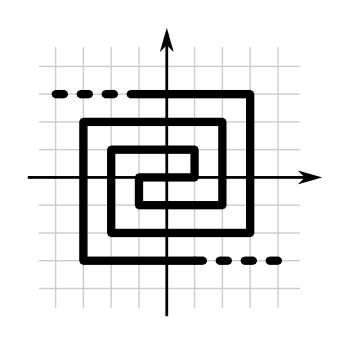
\includegraphics{spiral}
\end{center}
Here, $f(0)=(0,0)$, $f(1)=(1,0)$, $f(2)=(1,1)$, $f(3)=(1,0)$, etc. In fact, such
a bijection is also a group homomorphism. This is because the $a+b$-th
``position'' in the spiral is the same as taking $a$ steps along the spiral (in
the direction corresponding to the parity of $a$,) and then taking $b$ steps
along the spiral in the same way. We note that the identity is preserved (i.e.
$f(0)=(0,0)$.) Also, inverses are preserved. To see this, notice how
$f(a+1)-f(a)$ is opposite (in terms of parity) of $f(-a-1)-f(-a)$. This means
that $f$ as it maps $1,2,3,4$ ``mirrors'' itself as it maps along $-1,-2,-3,-4$.
You can check how, for instance, how $-f(6)=f(-6)$.
\end{solution}


% Problem 3.5
\begin{problem}
Prove that $\mathbb{Q}$ is not the direct product of two nontrivial groups.
\end{problem}
\begin{solution}
Let $(a,b),(c,d)\in\mathbb{Q}$. We know that $\mathbb{Q}$ isn't a direct product
because $(a,b)+(c,d)$ isn't equal to $(a+b,c+d)$, but $(ad+bc,cd)$. In
particular, the left hand side is in terms of four elements---$a,b,c,d$---two of
which being from the $G$ group and the second being from the $H$ group, whereas
the first component of the product two elements in a direct product group is
only in terms of two elements in $G$.
\end{solution}


% Problem 3.6
\begin{problem}
$\rhd$ Consider the product of the cyclic groups $C_2$, $C_3$ (cf. \S2.3):
$C_2\times C_3$. By Exercise 3.3, this group is a coproduct of $C_2$ and $C_3$
in $\Ab$. Show that it is not a coproduct of $C_2$ and $C_3$ in $\Grp$, as
follows:
\begin{itemize}
\item find injective homomorphisius $C_2\to S_3, C_3\to S_3$;
\item arguing by contradiction, assume that $C_2\times C_3$ is a coproduct of
$C_2$, $C_3$, and deduce that there would be a group homomorphism $C_2\times
C_3\to S_3$ with certain properties;
\item show that there is no such homomorphism.
\end{itemize}
\end{problem}
\begin{solution}
Consider $C_2,C_3,S_3$. We can construct injective morphisms $f_{C_2}$ and
$f_{C_3}$ as follows:
%
\[ f_{C_2}([a]_2) = \sigma^a_2 \]
\[ f_{C_3}([a]_3) = \sigma^a_3 \]
%
(using the cyclic permutation construction, $\sigma_d\in S_n$ with $d\leq n$ and
$\abs{\sigma_d}=d$, from above.) 

Suppose $C_2\times C_3$ is a coproduct in $\Grp$ with morphisms
$\iota_{C_2}:C_2\to C_2\times C_3$ and $\iota_{C_3}:C_3\to C_2\times C_3$.
Considering $S_3$ with $f_{C_2}$ and $f_{C_3}$, by the universal property of
coproducts there is a unique morphism $\varphi:C_2\times C_3\to S_3$ such that
$\iota_{C_2}\varphi = f_{C_2}$ etc.

Since $f_{C_2}$ and $f_{C_3}$ are injective, all of $\iota_{C_2}$,
$\iota_{C_3}$, and $\varphi$ must be injective.  (To see this, suppose
$\iota_{C_2}$ isn't injective; then $\iota_{C_2}([a]_2) = \iota_{C_2}([b]_2$ for
$a\neq b$, which means that $\varphi\iota_{C_2}([a]_2) =
\varphi\iota_{C_2}([b]_2)$; however, this cannot be, since the diagram must
commute with the injective function $f_{C_2}$.)

Now, notice that $S_n$ has three elements of order 2 (the ``reflection''
elements,) while $C_2$ has one, $([1]_2,[0]_3)$. This means that there must be a
$g\in C_2\times C_3$ such that $\abs{g}>2$ but $\abs{\varphi(g)}=2$. But this
means that $\varphi(\inv{g})=\varphi(g)$, even though (since $\abs{g}>2$,)
$g\neq\inv{g}$. Hence $C_2\times C_3$ is not a coproduct in $\Grp$.
\end{solution}

\end{document}
